\section{Formal semantics}

\subsection{Rationale}

\frame {
  \frametitle{Why formal semantics}
  \begin{itemize}
    \item Allow a mathematical treatment of the system under
      consideration
    \item Allow reasoning based on the mathematical model
    \item We used Structured Operational Semantics (SOS)
    \item SOS describes system evolution as transitions
    \item Each transition has \alert{antecedents} and
      \alert{consequents}
    \item Antecedent describe the preconditions for transition
    \item Consquents describe the transition itself
  \end{itemize}
}

\subsection{Static semantics and Ravenscar Meta-model}

\frame {
  \frametitle{Static semantics}
  \begin{itemize}
    \item Gives the rules for the well-formedness of entities
    \item Uses set theory concepts to describe the entities
    \item The static semantics corresponds to the RMM
  \end{itemize}
  
  \begin{minipage}{0.45\linewidth}
    {\footnotesize
      \begin{eqnarray}
        \nonumber
        \text{\textbf{Periodic tasks}} \ {\cal T}_p \!& \!= \!&\! \{P_1 \ldots P_n\}\\
        \nonumber
        \text{\textbf{Sporadic tasks}} \  {\cal T}_s  \! & \!= \! & \!  \{S_1  \ldots S_m\} \\
        \nonumber
        \text{\textbf{Interrupts}} \   {\cal U} \! & \!= \! & \! \{U_1  \ldots U_k\}  \\ 
        \nonumber
        \text{\textbf{Synchronisers}} \    {\cal D} \! & \!= \! & \! \{D_1 \ldots D_l\} \\  
        \nonumber
        \text{\textbf{Exchangers}} \  {\cal E} \! & \!= \! & \! \{E_1  \ldots E_r\} 
      \end{eqnarray}
    }
  \end{minipage}
  \hspace{2mm}
  \begin{minipage}{0.45\linewidth}
    {\footnotesize
      \begin{eqnarray}
        \nonumber
        \text{\scshape priority}: &{\cal C} & \to \ \ 
             {\scriptstyle \mathbb{ANYPRIORITY}} \\
        \nonumber
        \text{\scshape holdingtime}: & {\cal T} & \to \ \  
             {\scriptstyle \mathbb{TIME}} \\
        \nonumber
        \text{\scshape wcet}: & {\cal A}  &  \to \ \  
             {\scriptstyle \mathbb{TIME}} \\
        \nonumber
        \text{\scshape deadline}: & {\cal A}   &  \to  \ \  
             {\scriptstyle \mathbb{TIME}} \\
        \nonumber
        \text{\scshape prog}: & {\cal C}  & \to \ \  
             {\scriptstyle \mathbb{PROGS}} 
      \end{eqnarray}
    }
  \end{minipage}
}

\frame {
  \frametitle{RMM}
  \begin{center}
    $\includegraphics[scale=0.4]{../figs/rmm}$
  \end{center}
}

\frame {
  \frametitle{Topological definitions}
  {\footnotesize
  \begin{eqnarray}
    \nonumber
    \text{\emph{sets}} & : & \rset \ \subset\  \ {\cal A} \times {\cal
      E} \\
    \nonumber
    \text{\emph{gets}} & : & \rget \ \subset \ \ {\cal T} \times {\cal
      E}  \\
    \nonumber
    \text{\emph{sends\_event}} & : &  \rsvt \  \subset \ \ {\cal A}
    \times {\cal D} \\
    \nonumber
    \text{\emph{awaits\_event}} & : &  \rgvt \ \subset \ \ {\cal T}_s
    \times {\cal D}
  \end{eqnarray}
  }
}

\subsection{Dynamic semantics \& system evolution}

\frame {
  \frametitle{Structured Operational Semantics}
  \begin{itemize}
    \item Labelled transition system
    \item Has preconditions to describe system state that exists
    \item Takes an action, changes system variables (from static
      semantics)
    \item Reaches a new state
  \end{itemize}
  \pause
  \begin{center}
    {\footnotesize
    \formatreg{
      \regle{ \textit{Antecedents}}
	    {
	      \text{\small  \textit{IL}} \intrupt 
	      \big[ 
	        c, R, B, \text{\sffamily ns}, \text{\sffamily t} 
	        \big]
	      \Faitv{\textit{act}}
	      \text{\small  \textit{IL'}} \intrupt
	      \big[ 
	        c', R,' B', \text{\sffamily ns'}, 
	        \text{\sffamily t}
	        \big] \sqplus \delta(\textit{\small act})
	    } \textit{\scriptsize SHORT NAME}
    }
    }
  \end{center}
}

\frame {
  \frametitle{Example transition}
  Models the preemption by the scheduler of a task that is \emph{not}
  the idle task\\

  \formatreg {
    \regle {
      c\neq\iota\ \wedge\ c\neq \sigma\ \wedge\ c\neq
      \sigma_s\ \wedge\ c=a\ \wedge\ \text{\sffamily t}=\text{\sffamily ns} 
    } {
      \big[c, R, B, \text{\sffamily ns}, 
        \text{\sffamily t} 
        \big]
      \Faitv{\text{as}}
      \big[ 
        \sigma, R', B, \text{\sffamily ns}, 
        \text{\sffamily t}
        \big]
      \sqplus 
      \delta(as)\\
      \\
      R' = a\smcirc R
    }
  }
}
